\documentclass{paper}

%\usepackage{times}
\usepackage{epsfig}
\usepackage{graphicx}
\usepackage{mathtools}
\usepackage{amssymb}
\usepackage{color}
\usepackage{caption}
\usepackage{subcaption}
\usepackage{natbib}
\usepackage{url}
\usepackage{hyperref}
% load package with ``framed'' and ``numbered'' option.
%\usepackage[framed,numbered,autolinebreaks,useliterate]{mcode}

% something NOT relevant to the usage of the package.
\setlength{\parindent}{0pt}
\setlength{\parskip}{18pt}






\usepackage[latin1]{inputenc} 
\usepackage[T1]{fontenc} 

\usepackage{listings} 
\lstset{% 
   language=Matlab, 
   basicstyle=\small\ttfamily, 
} 



\title{Report for assignment 3}



\author{Moser Stefan\\09-277-013}
% //////////////////////////////////////////////////


\begin{document}



\maketitle

\section{Video search with bags of visual words (Due on 17/12/2013)}
In this assignment we studied how well SIFT descriptors perform when used directly 
for matching and in combination with bag of words. As underlying data set I used the
one provided with the assignment (Two frames from one scene of an episode of the TV series 'Friends',
see twoFrameData.mat) and 33 frames extracted from various scenes of one episode of the
British TV series 'Doctor Who' (see the folder /images provided with the code or Figure \ref{fig:db}). The
frames were extracted using VLC media player\footnote{\url{http://www.videolan.org/vlc/}},
partly with subtitles.
The computation of the SIFT descriptors and the clustering were done with the VLFeat\footnote{\url{http://www.vlfeat.org/}} open source library.

\subsection{Experiments}
\subsubsection{Raw descriptor matching}
\label{sec:raw}
For this experiment, the user selects a region of interest on one frame. Every 
descriptor contained in this region is then mapped to a descriptor in a second frame.
The assumption is, that the descriptors found on an object only vary negligible along
multiple frames. This does work reasonably well as can be seen
on Figure \ref{fig:raw_desc_match}. My algorithm does not prevent two descriptors from
frame 1 being matched to the same descriptor on frame 2. This behavior was chosen for
 algorithmic simplicity and runtime performance. Another approach would be to exclude 
the descriptor from further matching after it was assigned once.
This simple algorithm is very easy to throw off as can be seen in Figure \ref{fig:raw_fail}.
\begin{figure}
  \centering
  \begin{subfigure}[b]{0.7\textwidth}
    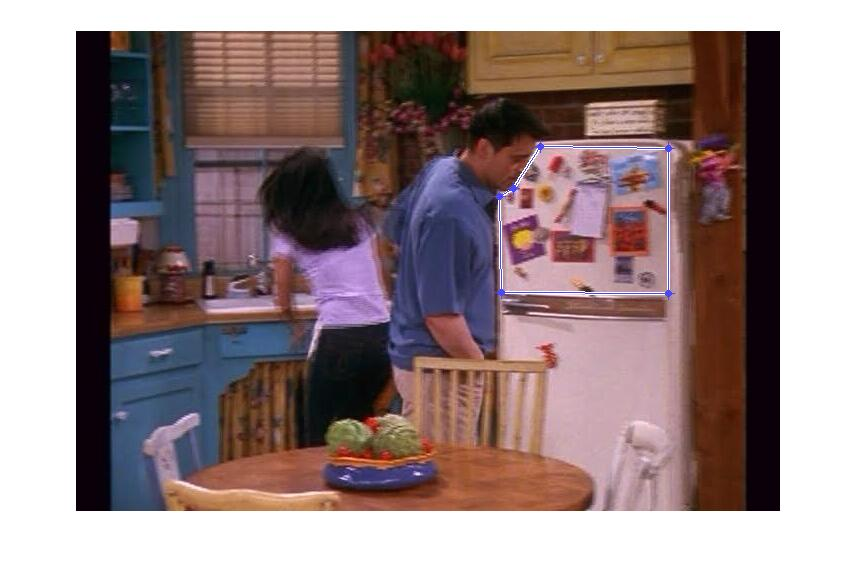
\includegraphics[width=\textwidth]{raw_desc_matching_selection}
    \subcaption{Selected region on frame 1: The fridge}
  \end{subfigure}
  \begin{subfigure}[b]{0.7\textwidth}
    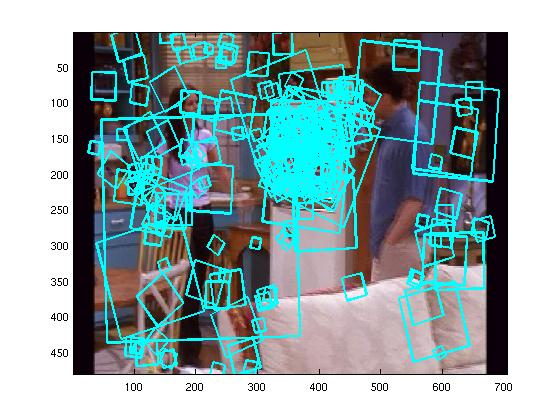
\includegraphics[width=\textwidth]{raw_desc_matching_all}
    \subcaption{All matched descriptors on frame 2. MSE: 0.325343}
  \end{subfigure}
    \begin{subfigure}[b]{0.7\textwidth}    
    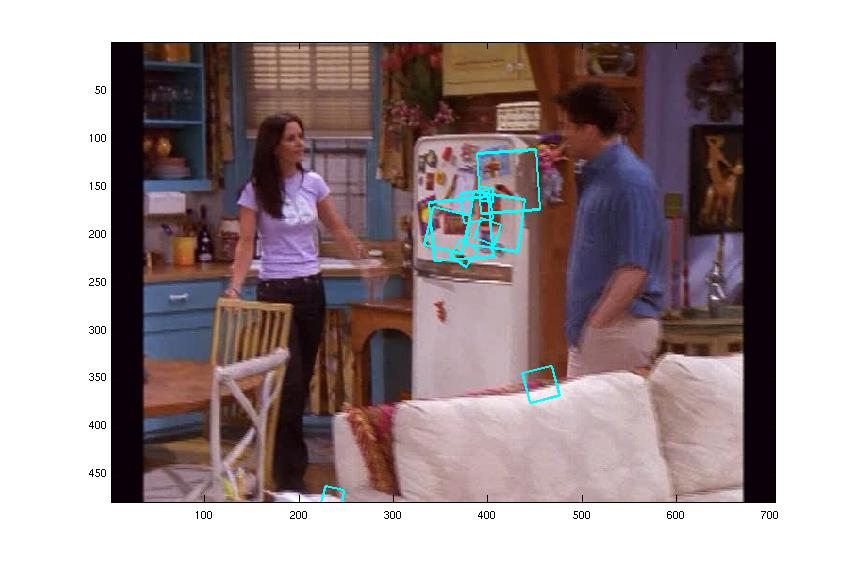
\includegraphics[width=\textwidth]{raw_desc_matching_topten}
    \subcaption{Selection of 10 best matches on frame 2. MSE: 0.087385}
  \end{subfigure}
\caption{Raw descriptor matching of the provided scene. When displaying all matches,
the result seems very disappointing. When only including the best matches, most 
descriptors lie on the initially selected object.}
\label{fig:raw_desc_match}
\end{figure}
\begin{figure}
  \centering
  \begin{subfigure}[b]{0.7\textwidth}
    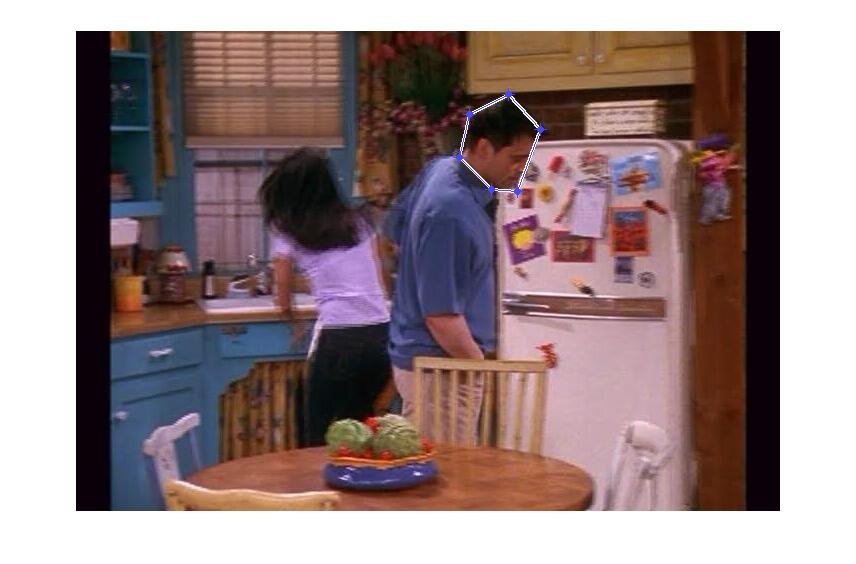
\includegraphics[width=\textwidth]{raw_fail_selection}
    \subcaption{Selected region on frame 1: Joey's head}
  \end{subfigure}
  \begin{subfigure}[b]{0.7\textwidth}
    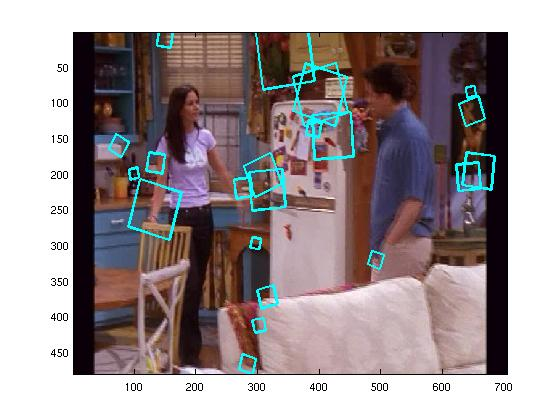
\includegraphics[width=\textwidth]{raw_fail_all}
    \subcaption{All matched descriptors on frame 2. MSE: 0.368444}
  \end{subfigure}
\caption{Another example of raw descriptor matching of the provided scene.
In this example, the matched descriptors do not lie in the expected region, even though
the mean square error is close to the one of the first example}
\label{fig:raw_fail}
\end{figure}

\subsection{Visualizing the visual vocabulary}
For this example we compile a visual vocabulary: We compute the SIFT features of every 
frame in our database, concatenate all of them and apply clustering via the k-means 
algorithm. Every SIFT patch assigned to the same center (or 'word') can then be 
seen as representation of this word. For my data set, a histogram of all assignments can be
seen in Figure \ref{fig:all_hist}. Some sample representations are visualized in Figure 
\ref{fig:words}. As my data set contains images that have a large portion covered with sky,
which consists of mainly uniform patches, all descriptors in these regions are mapped to
the same word, which is apparently number 65. The similarity of the patches for the two 
other words is not as easy to see by human eyes. They do however share similar gradient
directions in similar subregions, which is essentially what is expressed by SIFT. 

Contrary to intuition, we can also spot several mostly uniform patches in word 949
(Figure \ref{fig:949}). When normalizing these patches however, they show similar 
gradient directions as the other representatives of word 949. They are just too weak to see
by eye. Since SIFT does not consider the magnitude of the gradient but only its direction,
they show up under the same word. We can however adapt SIFT to either ignore every 
gradient that has a magnitude below a threshold or classify these below a threshold as 
special null-direction. For computing the results shown in Figure \ref{fig:words} I 
choose the former behavior with 10 as threshold. 
Without this tweak, there would be even more mostly uniform patches scattered in other words,
which does not serve our purpose.
\begin{figure}
  \centering
  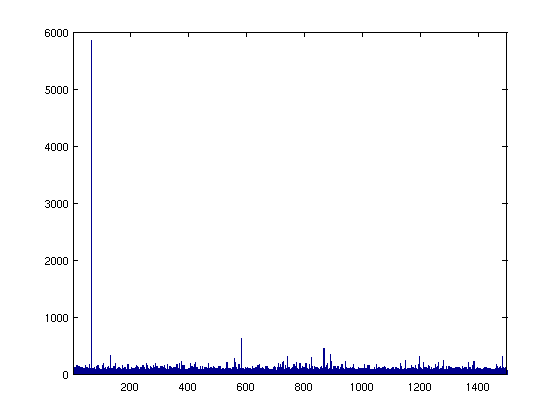
\includegraphics[width=0.7\textwidth]{hist_all}
  \caption{Histogram of the assignments for all descriptors in database. It becomes 
  apparent that word 65 is by far the most prominent word.}
  \label{fig:all_hist}
\end{figure}
\begin{figure}
  \centering
  \begin{subfigure}[b]{0.32\textwidth}
    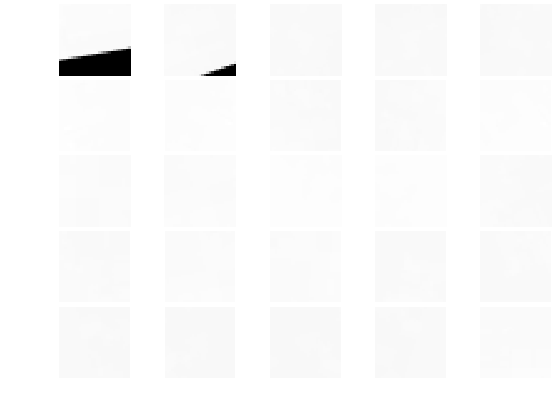
\includegraphics[width=\textwidth]{word65_uniform}
    \subcaption{Word 65}
    \label{fig:65}
  \end{subfigure}
  \begin{subfigure}[b]{0.32\textwidth}
    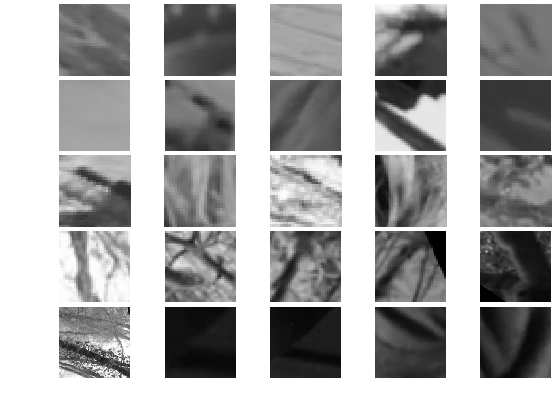
\includegraphics[width=\textwidth]{word147}
    \subcaption{Word 147}
  \end{subfigure}
    \begin{subfigure}[b]{0.32\textwidth}    
    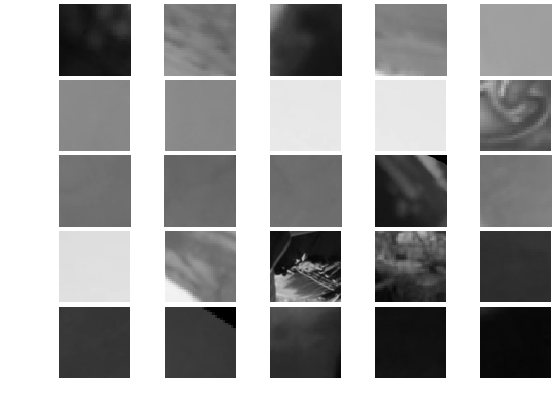
\includegraphics[width=\textwidth]{word949}
    \subcaption{Word 949}
    \label{fig:949}
  \end{subfigure}
\caption{Three different words their first 25 representatives. Word 65 from subfigure \subref{fig:65}
is the most common word, as can be seen in the histogram in Figure \ref{fig:all_hist}. It contains 
mostly uniform patches. The other two words are not as easy described.}
\label{fig:words}
\end{figure}
\subsection{Full frame queries}
After computing visual words, we can use these to specify similarity: If the words appear
in the same quantity on frame 1 as on frame 2, we assume them to contain the same objects
and to be similar. This can be computed by simply computing the normalized
 scalar product of the histograms of our 
query frame with each other frame and pick the highest values. Results obtained with this
method can be seen in Figure \ref{fig:full_frame_query}. 
\begin{figure}
  \centering
  \begin{subfigure}[b]{0.32\textwidth}
    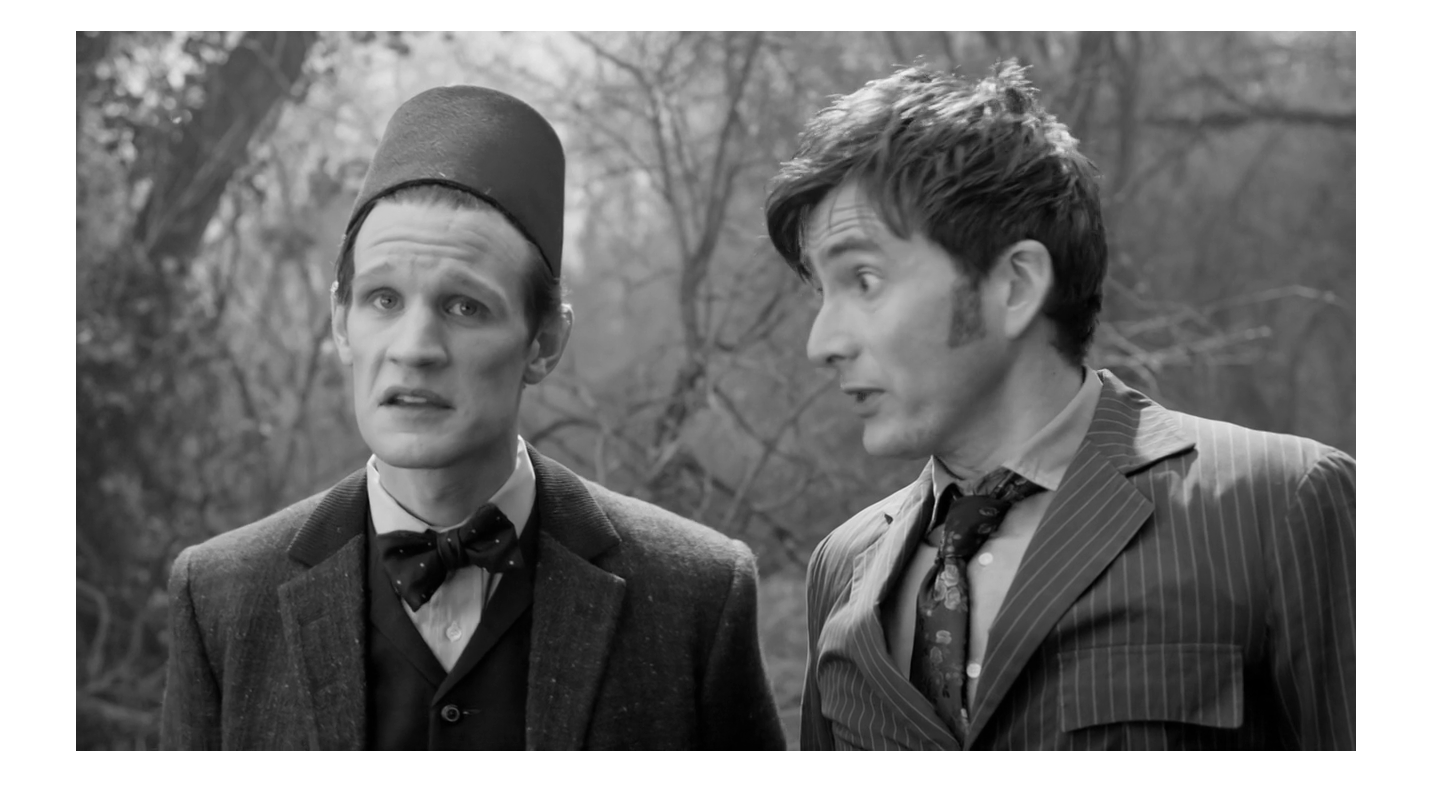
\includegraphics[width=\textwidth]{full_frame_query_img}
    \caption{Query image}
  \end{subfigure}
  \begin{subfigure}[b]{0.32\textwidth}
  	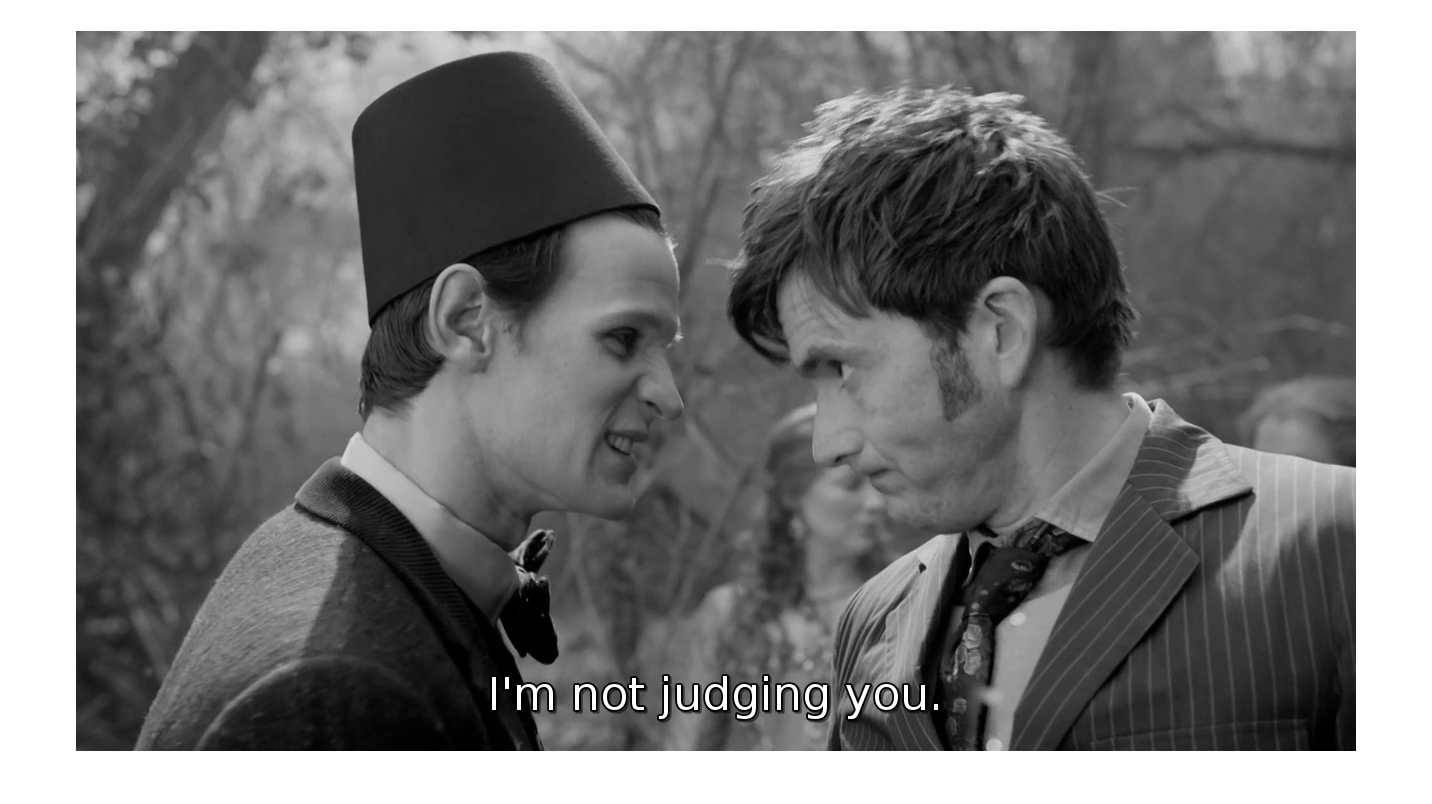
\includegraphics[width=\textwidth]{full_frame_query_result1}
  	\caption{Result 1}
  \end{subfigure}
  \begin{subfigure}[b]{0.32\textwidth}
  	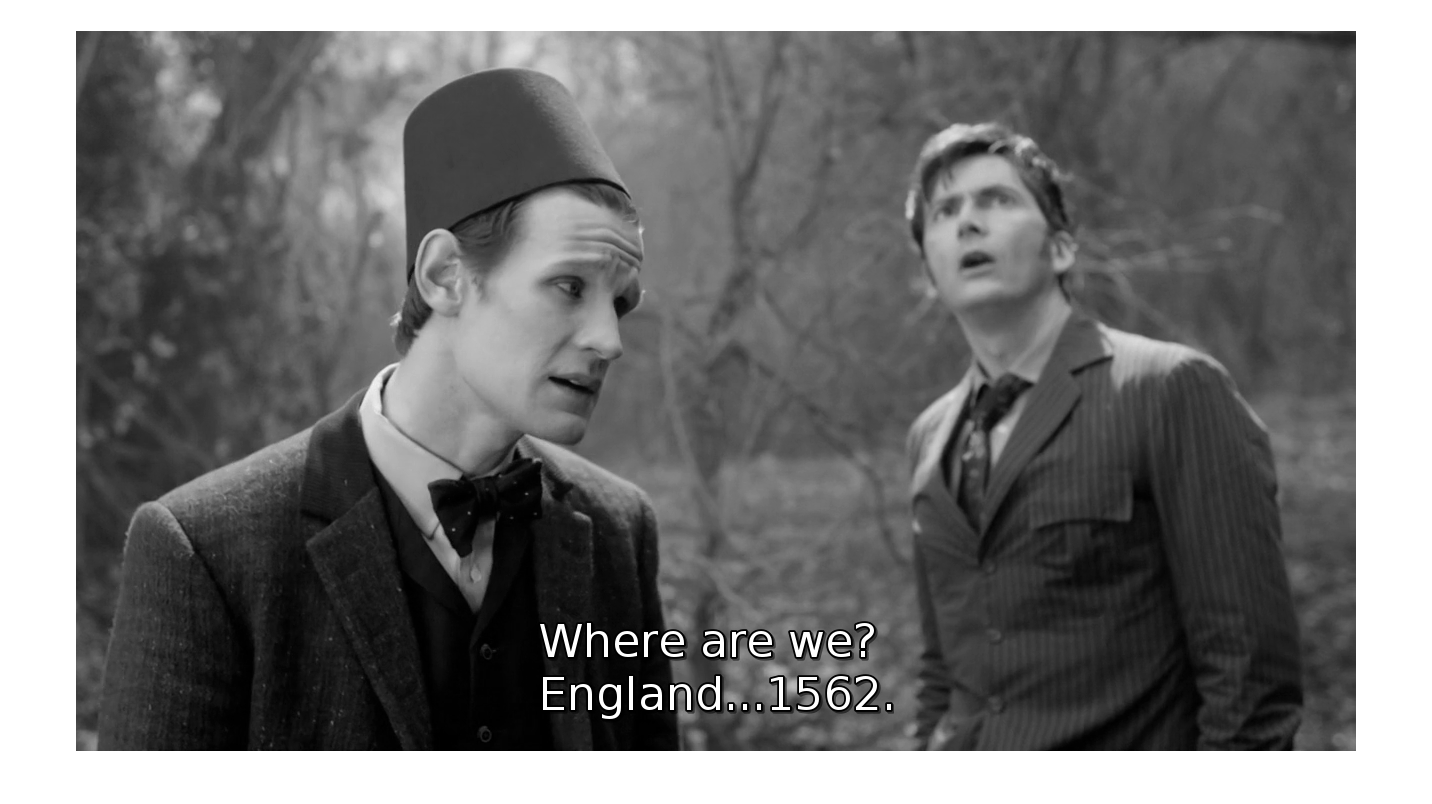
\includegraphics[width=\textwidth]{full_frame_query_result2}
  	\caption{Result 2}
  \end{subfigure}
  \begin{subfigure}[b]{0.32\textwidth}
  	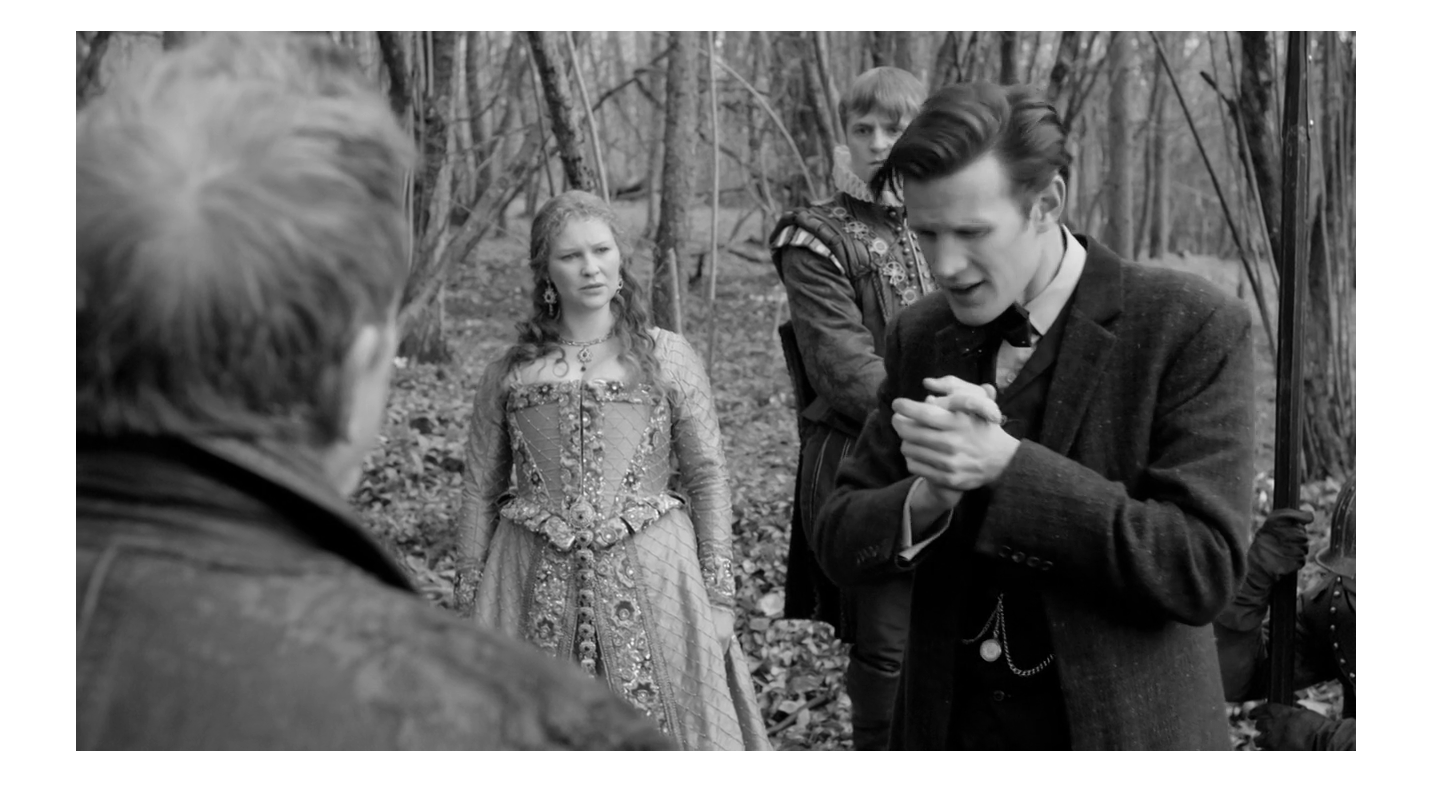
\includegraphics[width=\textwidth]{full_frame_query_result3}
  	\caption{Result 3}
  \end{subfigure}
  \begin{subfigure}[b]{0.32\textwidth}
  	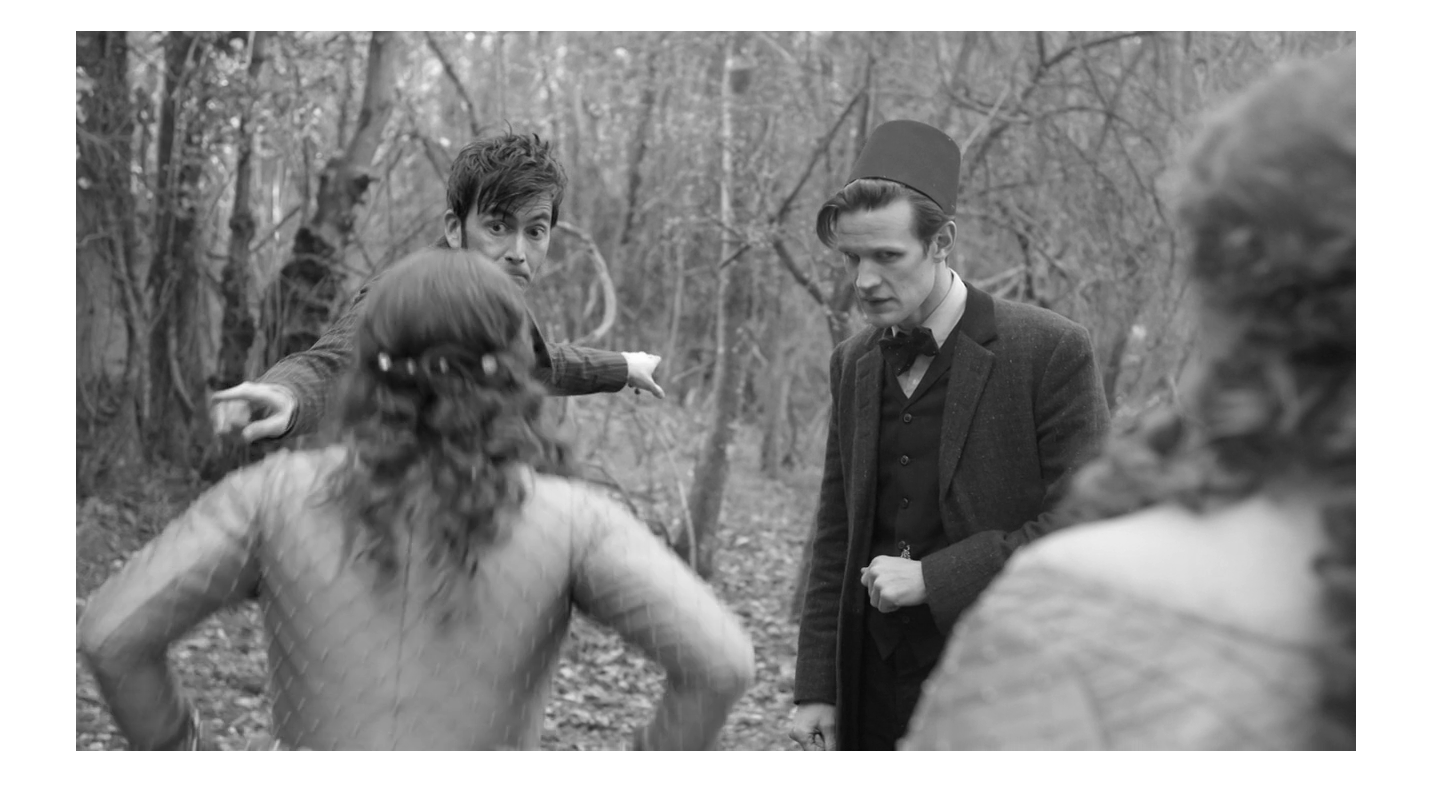
\includegraphics[width=\textwidth]{full_frame_query_result4}
  	\caption{Result 4}
  \end{subfigure}
  \begin{subfigure}[b]{0.32\textwidth}
  	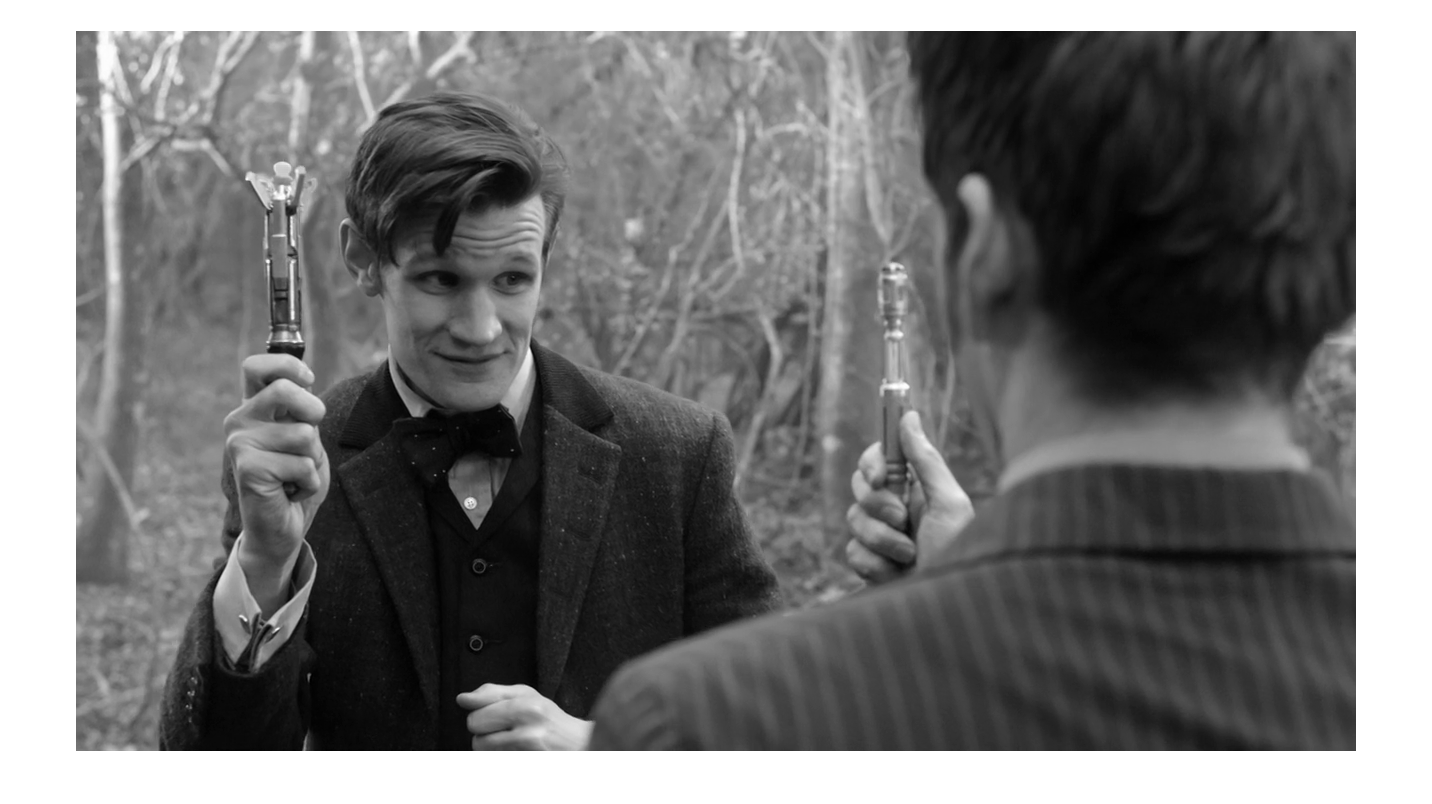
\includegraphics[width=\textwidth]{full_frame_query_result5}
  	\caption{Result 5}
  \end{subfigure}
  \caption{An example for a full frame query with results sorted by similarity. 
  The results are convincing: Frames that contain
  the same actors from the same scene are found. 
  Not even the subtitles confuse the algorithm.}
  \label{fig:full_frame_query}
\end{figure}
\subsection{Region query}
Similar to full frame query, we can also compute the histogram of words of a user 
selected region and us it in the same way for finding images that contain the 
selected region. Additionally we can weight the histogram of the selected region
using term frequency inverse document frequency (tf-idf). This lessens the impact
of omnipresent words by multiplying the log of the inverse document frequency:
\begin{equation}
	p'(w) = p(w) \cdot \log(\frac{|a|}{p_a(w)})
\end{equation}
In this equation $p(w)$ is the frequency of the word $w$ in the current frame and $p_a(w)$
 it's frequency over the whole database. $|a|$ is the number of descriptors in the 
 whole database. $p'(w)$ is the resulting weighted frequency of $w$.
 As in the last experiment, we use the normalized scalar product as similarity measure.
Two examples can be seen in Figure \ref{fig:region_qry_fez} and \ref{fig:region_qry_souffle}.
\begin{figure}
  \centering
  \begin{subfigure}[b]{0.8\textwidth}
    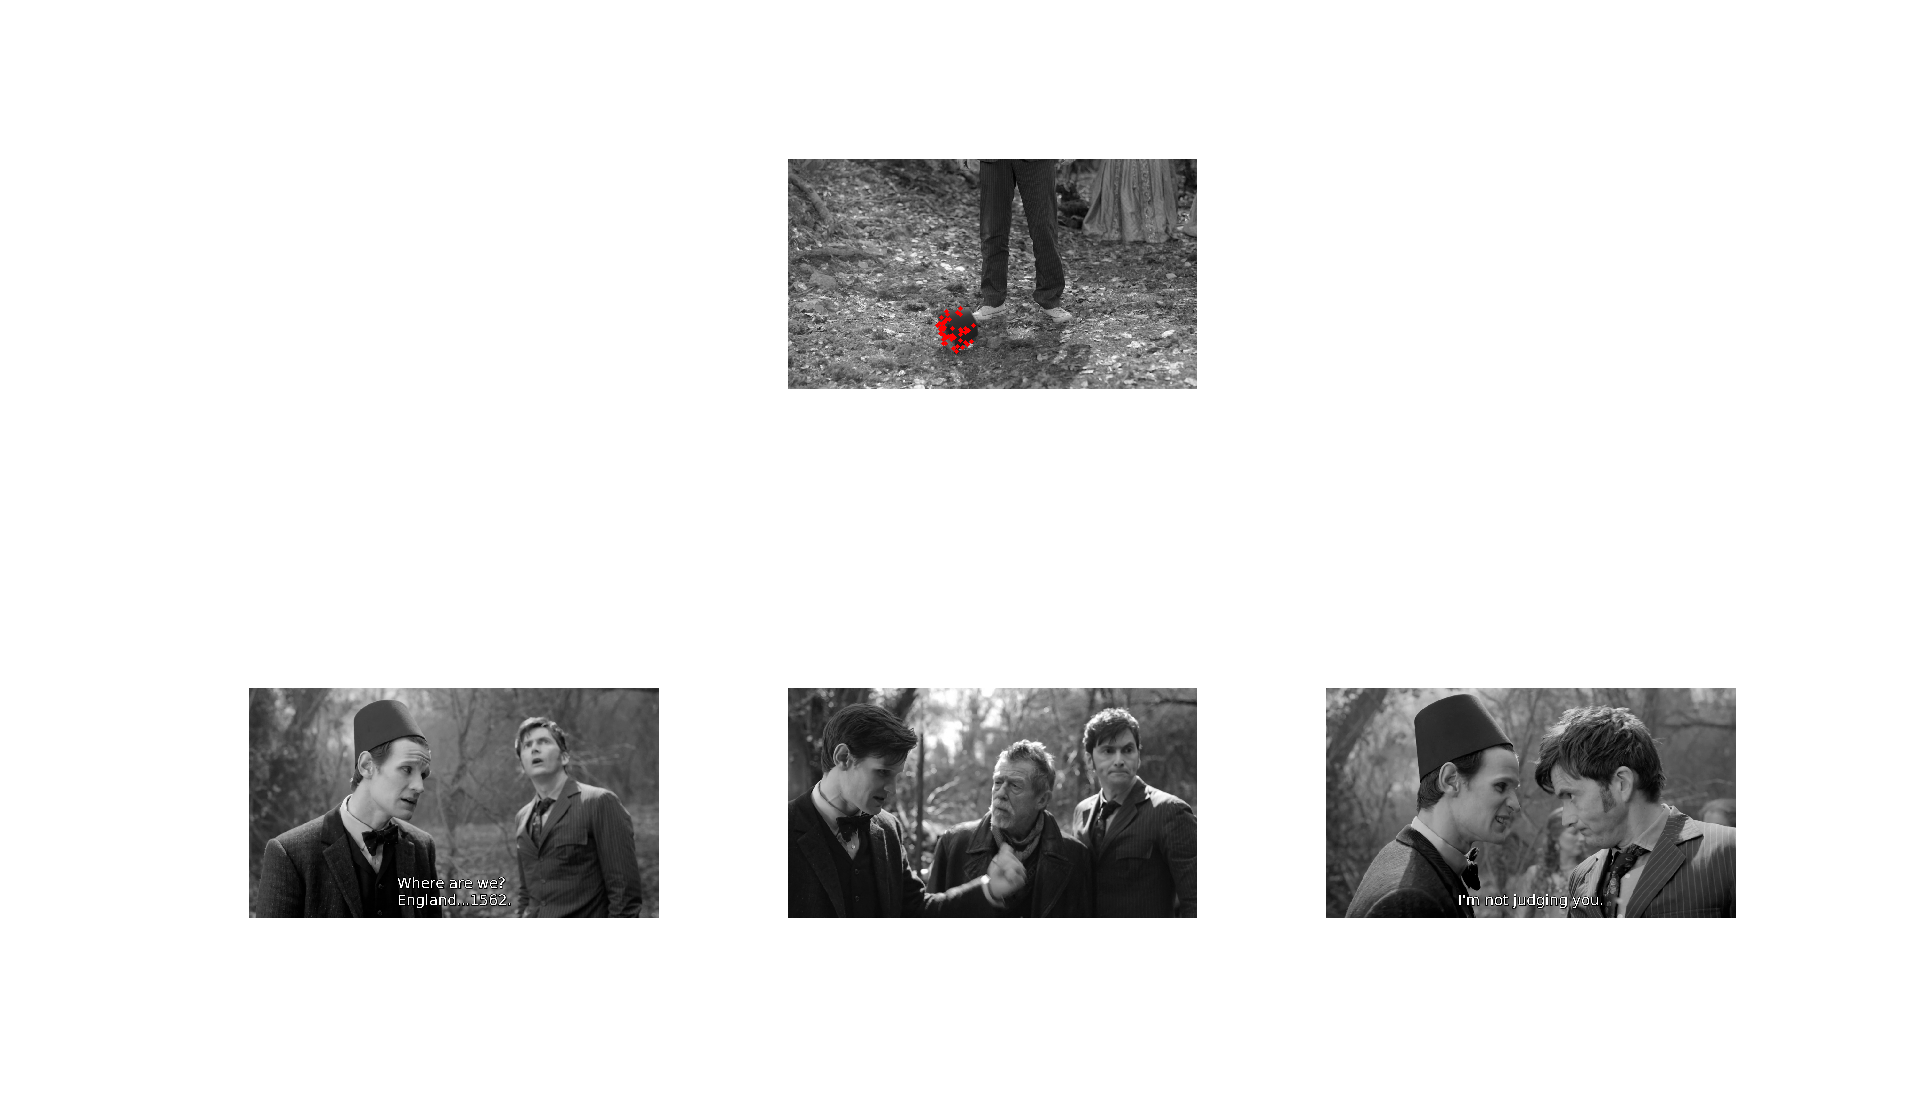
\includegraphics[width=\textwidth]{region_qry_fez}
    \subcaption{Descriptors in selected region are marked red on the upper
    image. The lower three images were determined as the most similar (in order 
    of similarity). The fez does indeed appear on the first and the third image.}
  \end{subfigure}
  \begin{subfigure}[b]{0.8\textwidth}
    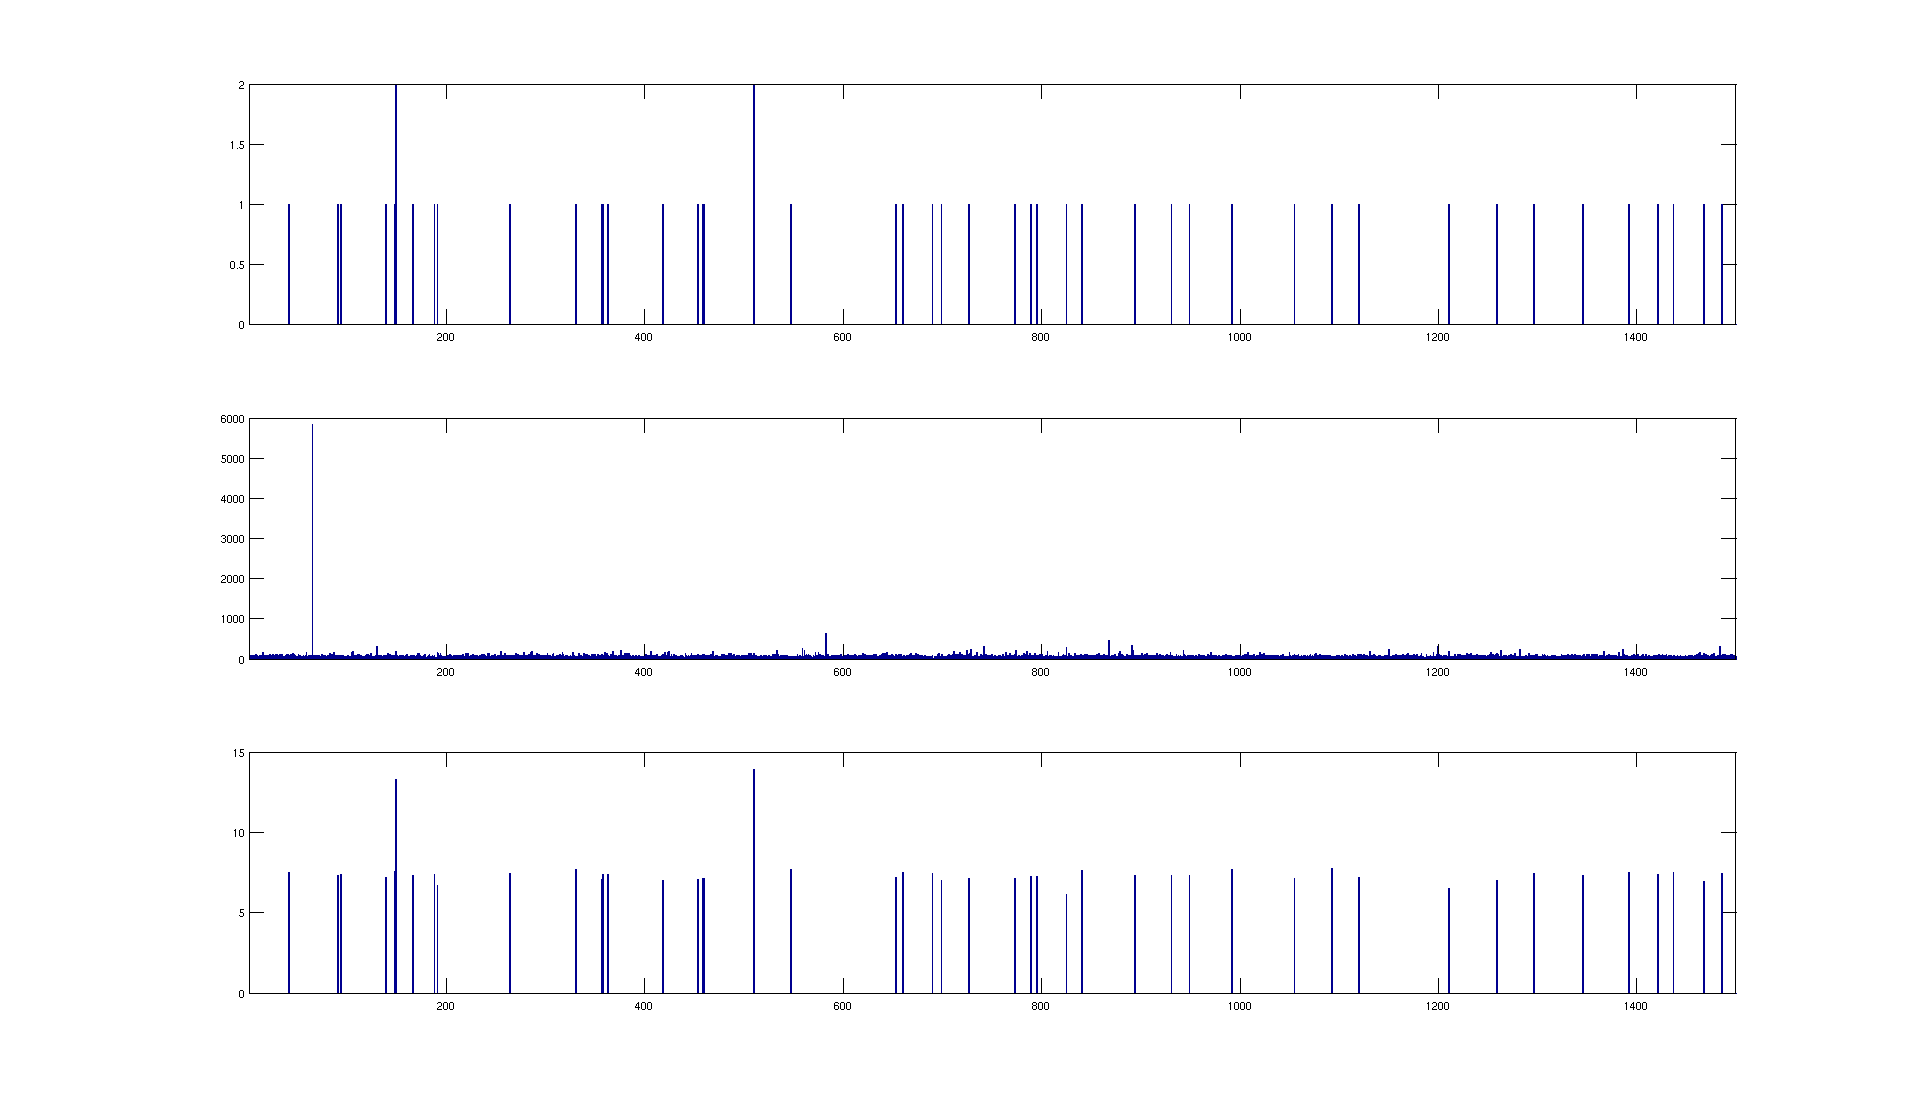
\includegraphics[width=\textwidth]{region_qry_fez_hist}
    \subcaption{At the top is the histogram of the selected region, in the middle
    the histogram over the whole database and at the bottom the histogram weighted
    with tf-idf.}
  \end{subfigure}
\caption{An example for a region query. The fez was selected as region of interest.}
\label{fig:region_qry_fez}
\end{figure}

\begin{figure}
  \centering
  \begin{subfigure}[b]{0.8\textwidth}
    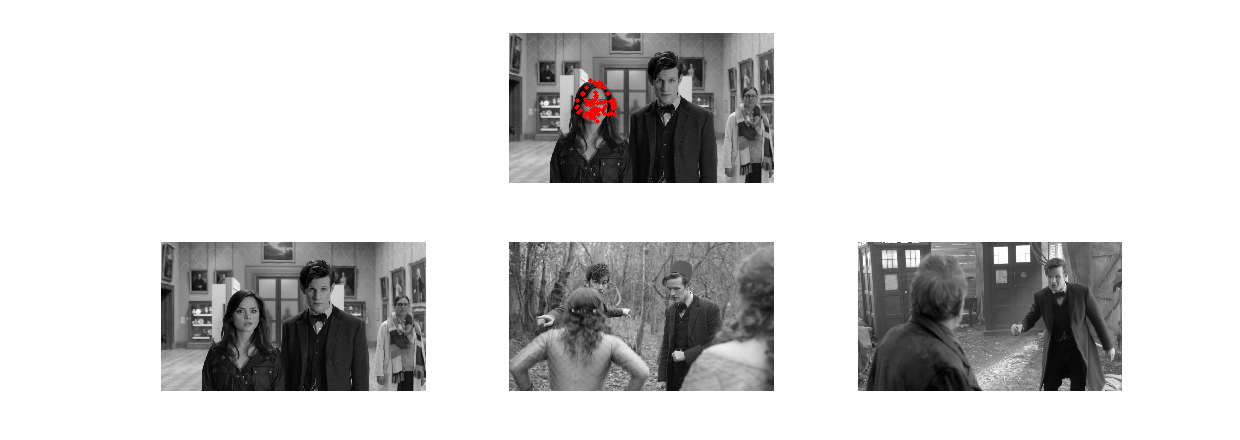
\includegraphics[width=\textwidth]{region_qry_souffle}
    \subcaption{Descriptors in selected region are marked red on the upper
    image. The lower three images were determined as the most similar (in order 
    of similarity). While the actress does appear on three other images of the database,
    even in front view, they are not found. At least the input image does show up.}
  \end{subfigure}
  \begin{subfigure}[b]{0.8\textwidth}
    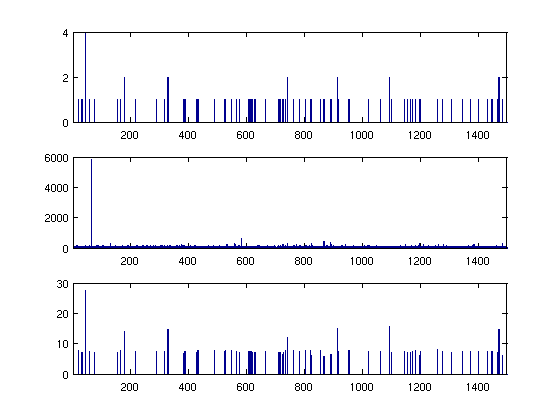
\includegraphics[width=\textwidth]{region_qry_souffle_hist}
    \subcaption{At the top is the histogram of the selected region, in the middle
    the histogram over the whole database and at the bottom the histogram weighted
    with tf-idf.}
  \end{subfigure}
\caption{A failure case for a region query. The face of the actress including hair
 was selected as region of interest.}
\label{fig:region_qry_souffle}
\end{figure}

\begin{figure}
  \centering
  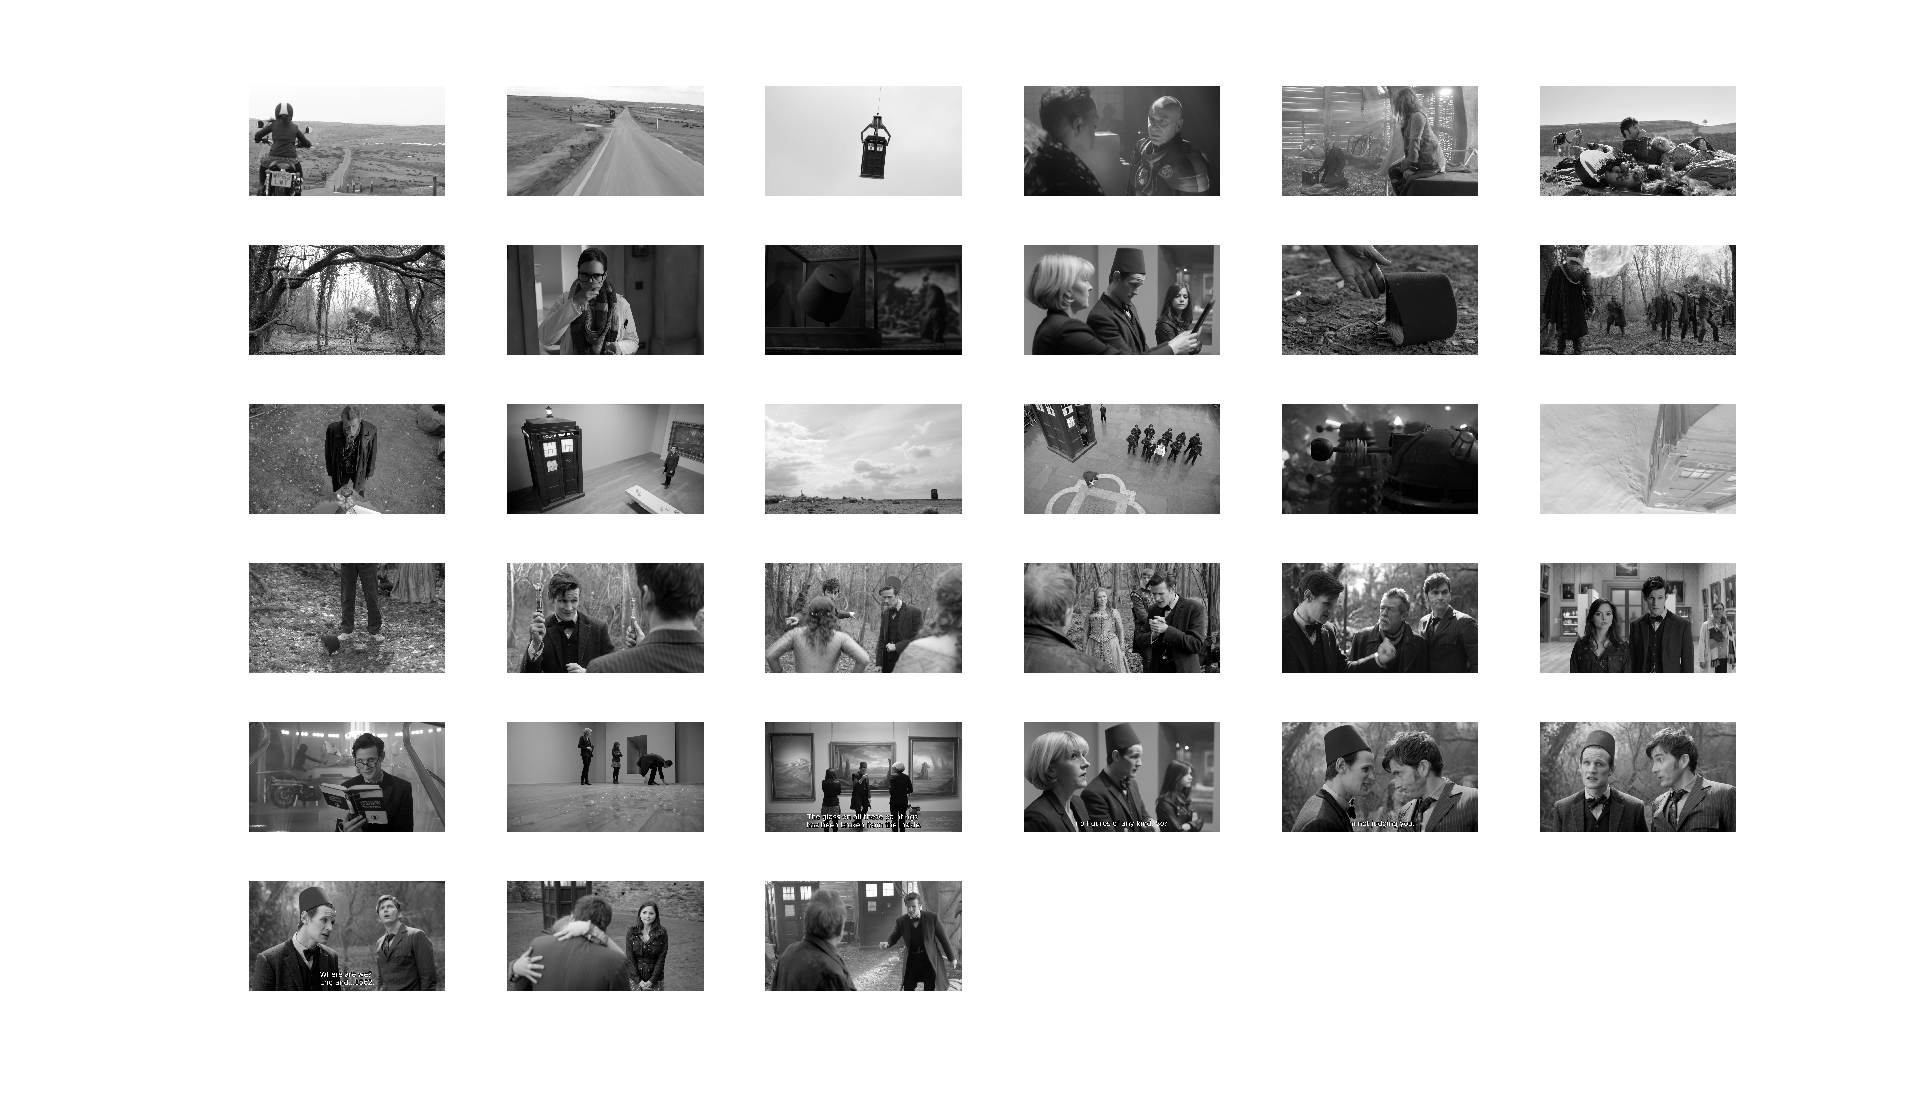
\includegraphics[width=\textwidth]{img_db}
  \caption{All images used for computing the results (except from section \ref{sec:raw}).}
  \label{fig:db}
\end{figure}
\end{document}